The data sets that are analyzed in this paper are MNIST and ORL. 

\subsection{ORL}
The ORL data set contains 400 vectorized images. The images are of size 40x30 and depict a persons face in an upright position in a frontal view\cite{orl_images}. There is 10 images of 40 different persons. Examples of the images can be seen on Figure \ref{fig:orl-images-raw}.

\begin{figure}[htbp]
    \centering
    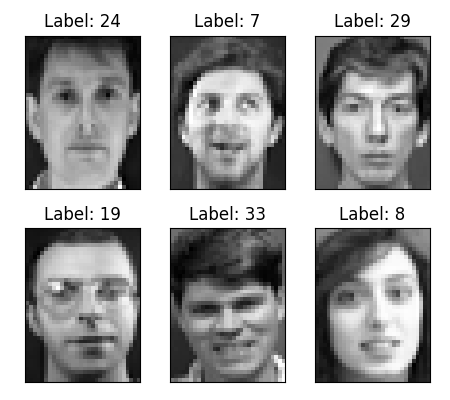
\includegraphics[width=0.7\columnwidth]{../source/orl/pictures/image-before-pca.png}
    \caption{ORL example images}
    \label{fig:orl-images-raw}
\end{figure}

\subsection{MNIST}
The MNIST dataset is larger with 70,000 vectorized images. The images depict handwritten digits and are of size 28x28. Differing from the ORL data set, the set is already split in training and test data. Leading to 60,000 images for training and 10,000 for testing. Examples from the MNIST data set can be seen on Figure \ref{fig:mnist-images-raw}.  

\begin{figure}[htbp]
    \centering
    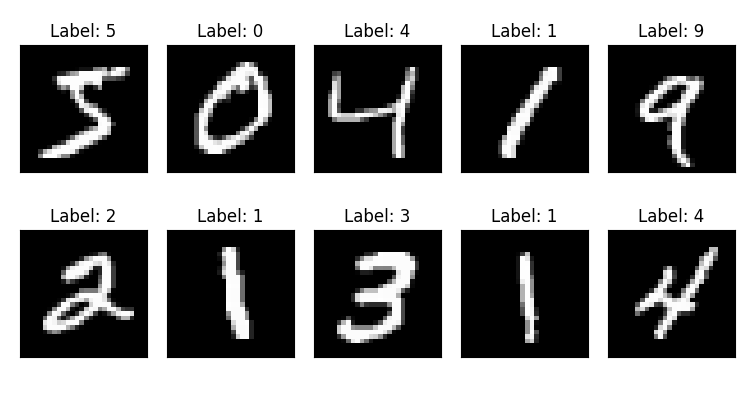
\includegraphics[width=0.7\columnwidth]{../source/mnist/pictures/image-before-pca.png}
    \caption{MNIST example images}
    \label{fig:mnist-images-raw}
\end{figure}